%%%%%%%%%%%%%%%%%%%%%%%%%%%%%%%%%%%%%%%%%
% Simple Sectioned Essay Template
% LaTeX Template
%
% This template has been downloaded from:
% http://www.latextemplates.com
%
% Note:
% The \lipsum[#] commands throughout this template generate dummy text
% to fill the template out. These commands should all be removed when 
% writing essay content.
%
%%%%%%%%%%%%%%%%%%%%%%%%%%%%%%%%%%%%%%%%%

%----------------------------------------------------------------------------------------
%	PACKAGES AND OTHER DOCUMENT CONFIGURATIONS
%----------------------------------------------------------------------------------------

\documentclass[12pt]{article} % Default font size is 12pt, it can be changed here

\usepackage{geometry} % Required to change the page size to A4
\geometry{a4paper} % Set the page size to be A4 as opposed to the default US Letter

\usepackage{graphicx} % Required for including pictures

\usepackage{float} % Allows putting an [H] in \begin{figure} to specify the exact location of the figure
\usepackage{wrapfig} % Allows in-line images such as the example fish picture

\usepackage{lipsum} % Used for inserting dummy 'Lorem ipsum' text into the template

\linespread{1.2} % Line spacing

%\setlength\parindent{0pt} % Uncomment to remove all indentation from paragraphs

\graphicspath{{Pictures/}} % Specifies the directory where pictures are stored

\begin{document}
	
	%----------------------------------------------------------------------------------------
	%	TITLE PAGE
	%----------------------------------------------------------------------------------------
	
	\begin{titlepage}
		
		\newcommand{\HRule}{\rule{\linewidth}{0.5mm}} % Defines a new command for the horizontal lines, change thickness here
		
		\center % Center everything on the page
		
		\textsc{\LARGE Wits University}\\[1.5cm] % Name of your university/college
		\textsc{\Large School of Electrical and Information Engineering}\\[0.5cm] % Major heading such as course name
		\textsc{\large ELEN7046 - Software Technologies and Techniques}\\[0.5cm] % Minor heading such as course title
		
		\HRule \\[0.4cm]
		{ \huge \bfseries Big Data Visualization using Commodity Hardware and Open Source Software}\\[0.4cm] % Title of your document
		
		Individual Report: Twit-Con-Pro Solution
		
		\HRule \\[0.6cm]
	
		\begin{minipage}
			{0.4
				\textwidth} 
			\begin{flushleft}
				\large \emph{Author:}\\
				Sidwell \textsc{Mokhemisa} \\
			\end{flushleft}
		\end{minipage}
		~ 
		\begin{minipage}
			{0.4
				\textwidth} 
			\begin{flushright}
				\large \emph{Student Number:} \\
				1229756 \\
				% Supervisor's Name
			\end{flushright}
		\end{minipage}
		\\[1cm]
		
			\
			\\
			\
			\\
			\
			\\
			\
			\\
			\
			\\
			Shared Project GitHub Repository:\\
			\
			https://github.com/garethstephenson/ELEN7046\_Group2\_2016\\
			\
			\\
			\
			\\
			\
			\\
			\
			\\
			\
			\\
			\
			\\
			
			{\large \today}\\[3cm] % Date, change the \today to a set date if you want to be precise
			
			%\includegraphics{Logo}\\[1cm] % Include a department/university logo - this will require the graphicx package
			
			\vfill % Fill the rest of the page with whitespace
			
				
	\end{titlepage}
	
		\newpage
		\begin{flushleft}\large
			\textsc{Declaration of Originality}\\
		\end{flushleft}
		
		I, Sidwell Mokhemisa, student number: 1229756, hereby declare the following:
		
		\begin{itemize}
			\item I am aware that plagiarism (the use of someone else’s work without their permission and/or without acknowledging the original source) is wrong.
			\item I confirm that ALL the work submitted for assessment for the above course is my own unaided work except where I have explicitly indicated otherwise.
			\item I have followed the required conventions in referencing the thoughts and ideas of others.
			\item I understand that the University of the Witwatersrand may take disciplinary action against me if there is a belief that this is not my own unaided work or that I have failed to acknowledge the source of the ideas or words in my writing.\\
			\\
			\\
		\end{itemize}
	
		\begin{figure}[H] % Example image
			\center{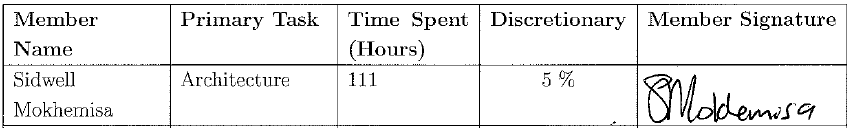
\includegraphics[width=1.15\linewidth]{Declaration1}}
			%\caption{IBM Rational Unified Process (Source: RUP, Best Practices for Software Development Teams)}
			\label{fig:speciation}
		\end{figure}
		
		
		\newpage
	
	
	% Abstract
	\begin{flushleft}\large
		\textsc{Abstract}\\
	%	XXXX.
		
	\end{flushleft}
%	{\large \today}\\[3cm] % Date, change the \today to a set date if you want to be precise
	
	%\includegraphics{Logo}\\[1cm] % Include a department/university logo - this will require the graphicx package
	
	\vfill % Fill the rest of the page with whitespace
	
	\newpage
	
	%	TABLE OF CONTENTS
	%----------------------------------------------------------------------------------------
	
	\tableofcontents % Include a table of contents
	
	\newpage % Begins the essay on a new page instead of on the same page as the table of contents 
	
	%----------------------------------------------------------------------------------------
	%	INTRODUCTION
	%----------------------------------------------------------------------------------------
	
	\section{Introduction} % Major section
	
This document covers a significant amount of deliverables that are key to the delivery of most projects that follow a formalized and structured software development lifecycle.
\\
\\
Deliverables covered in this topic are in the main architectural in nature with greater focus on High Level Design deliverables such as requirements, component model and Sequence Diagram(s) (Software Architecture), and Operational Model/ Physical Infrastructure Design.

% \subsection{Problem Statement}

% XXX

%\subsection{Solution Summary}

% XXX

\subsection{Approach}

The project shall be delivered by firstly trying to understand the requirements and modeling them into a set of Use-Cases which can then be used to direct the project from analysis to design, development, validation and verification, and benefits tracking once the system is taken into production and starts adding value to its end-users.

%\subsubsection{Methodology}
	
		%\subsection{Executive Summary} % --optional
		
		%------------------------------------------------
		
	\subsection{Background}
	This project was conceptualized to solve for a problem that is one of the key problems for both businesses and academic institutions as we move forward into this new world that is at the cutting edge of innovation and extreme levels of data available.
	
	The scope of the project shall be limited to acquiring data from Twitter (based on topic subscriptions - in this case, US and SA elections data for 2016), taking it through the process of transformation and analysis, and later making it available to users in a meaningful way using some of the cutting edge visualization tools that are relevent to solving the problem at hand.

	%	MAJOR SECTION 1
	\section{Lifecycle Methodology}
	
	The initial assessment of the project based on the project description and high level requirements showed the team that the project to be delivered can be classified as low-to-medium in terms of the classification scheme for projects based on the following broad categories:
	\begin{itemize}
		\item \textbf{Low -} This means the project to be delivered is classified as having low complexity and either small/ small-to-medium in terms of the budget and size of the delivery team.
		\item \textbf{Medium -} This means the project is classified as having medium complexity with medium budget and delivery team-size.
		\item \textbf{High -} This mean that the project is classified as being fairly complex, and requiring a huge budget and workforce for the success of its delivery.
	\end{itemize}
	
	It was for the reason of small-to-medium classification that the project followed a formal, plan-driven approach for the delivery of this project, based on IBM RUP with tailoring in order to make a determination/ up-front decision regarding the artifacts that were to be de-scoped, delivered at a level of detail sufficient to allow for the next phase(s) to continue, or to deliver a comprehensive artifact.
	\\
	\\
	The diagram below depicts the IBM RUP model[1]:
	
		\begin{figure}[H] % Example image
			\center{\includegraphics[width=1.15\linewidth]{ibm1}}
			\caption{IBM Rational Unified Process (Source: RUP, Best Practices for Software Development Teams)}
			\label{fig:speciation}
		\end{figure}
	
		\section{Assumptions and Constraints}
		
		\textbf{Assumptions:}
		
		The key assumptions made for this project are as follows:
		
		\begin{itemize}
			\item It is assumed that all the resources required to deliver this project are available and will be dedicated to the project from inception to transition.
			\item It is also assumed that the infrastructure planned for this initiative will be able to cater for the anticipated volumes.
		\end{itemize}

		\textbf{Constraints:}
		
		The following are the constraints identified during High Level Design:
		\begin{itemize}
			\item Limitation of the source system for the provision of social media and location data for non-commercial purposes.
			\item Time related constraints for the delivery of a working solution by the end date.	
		\end{itemize}
		
		\section {Design Decisions}
		
	The key design decision that was made in this project related to the tailoring of RUP artifacts in order to ensure success in the delivery while pitching the content of the deliverables at a sufficient level of detail to enable down-stream teams to continue with their work.
	\\
	\\
	The other major decision made was that of allowing for development as well as parts of production systems to run independent from each other and at different geographical areas to ensure continuity, and contribute to project service level characteristics of high availability and disaster recovery, albeit, not fully disaster recovery proof. 
	
    \section{Requirements - Use Case Models}
  
  The key Use Cases as identified by the project are discussed in this section.
    	
    \subsection{View Elections Analytic Data}
    
    This section covers the details around the visualization Use Case. The diagram below depicts the actual Use Case followed by a table that further discusses the Use Case details:
    
    	\begin{figure}[H] % Example image
    		\center{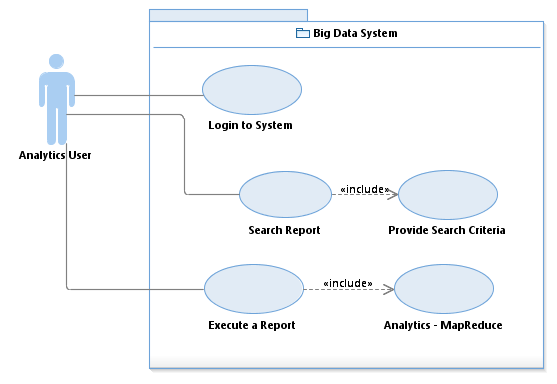
\includegraphics[width=1.0\linewidth]{UC01}}
    		\caption{Use Case Diagram - View Twitter Elections Analytics}
    		\label{fig:speciation}
    	\end{figure}
    	
  This table provides additional information to supplement the Use Case diagram.
   \begin{center}
   	\begin{tabular}{ | l | l | l | l |}
   		\hline
   		\multicolumn{1}{ |l| }{Use Case ID:} & \multicolumn{3}{| l |}{UC01}\\
   		\hline
   		\multicolumn{1}{|l|}{Use Case Name:} & \multicolumn{3}{|p{13cm}|}{View Analytics Social Media Report overlaid on map background.}\\
   		\hline
    	Created By: & Sidwell & Updated By: & Sidwell\\
    	\hline
    	Date Created: & 02/05/2016 & Date Modified: & 07/05/2016\\
    	\hline
   	\end{tabular}
   \end{center}
   \
   \
   \begin{center}
      	\begin{tabular}{ | r | p{12cm} |}
      		\hline     	
      		Actor : & Analytics User \\
      		\hline
      		Description: & This use case describes how the user will use the system to run analytics based on social media data received from Twitter.\\
      		\hline
      		Pre-conditions: & Web browser opened and user logs onto the analytics site.\\
      		\hline
      		Post-conditions: & User views requested report overlaid on map background. Drill up/ down functionality provided by the application.\\
      		\hline
      		Normal Course: & 1.	Logon to the application.
      		2.	Search report from list of available reports
      		3.	Execute a report of choice\\
      		\hline
      		Frequency of Use: & \\
      		\hline
      		Alternative Courses: & None\\
      		\hline
      		Exceptions: & None\\
      		\hline
      		Includes: & 1.	Provide search criteria or Hashtag(s).
      		2.	System runs report using Map Reduce and parallel processing in order to produce report results.\\
      		\hline
      		Special Requirements: & 1.	Ad-hoc access using most browsers (IE, Chrome, Safari).\\
      		\hline
      		Assumptions:& 1.	User login based on access to computer with browser and not necessarily integration to an LDAP compliant system.
      		2.	Support for mobile apps once developed.\\
      		\hline
      		Notes and Issues: & \\
      		\hline
      	\end{tabular}
      \end{center}
   
   \subsection{Acquire Twitter Data}
	
	This section covers the details around the data acquisition Use Case. The diagram below depicts the actual Use Case followed by a table that further discusses the Use Case details:
	
		\begin{figure}[H] % Example image
			\center{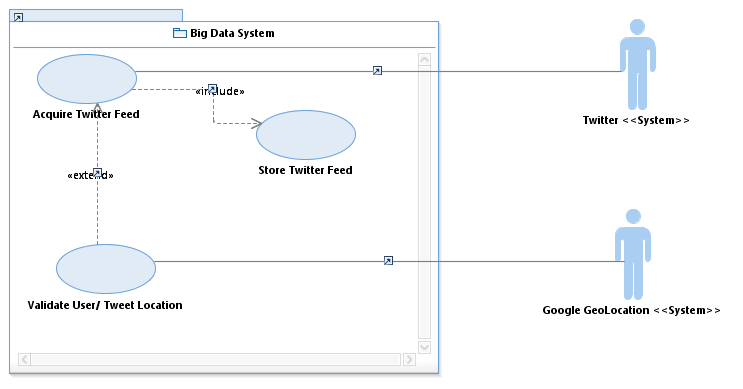
\includegraphics[width=1.0\linewidth]{UC02}}
			\caption{Use Case Diagram - Acquire Twitter Data}
			\label{fig:speciation}
		\end{figure}
		
	 This table provides additional information to supplement the Use Case diagram.
	  \begin{center}
	  	\begin{tabular}{ | l | l | l | l |}
	  		\hline
	  		\multicolumn{1}{ |l| }{Use Case ID:} & \multicolumn{3}{| l |}{UC02}\\
	  		\hline
	  		\multicolumn{1}{|l|}{Use Case Name:} & \multicolumn{3}{|p{13cm}|}{Acquire social media feed from twitter to enable big data analytics.}\\
	  		\hline
	  		Created By: & Sidwell & Updated By: & Sidwell\\
	  		\hline
	  		Date Created: & 02/05/2016 & Date Modified: & 07/05/2016\\
	  		\hline
	  	\end{tabular}
	  \end{center}
	  \
	  \
	  \begin{center}
	  	\begin{tabular}{ | r | p{12cm} |}
	  		\hline
	  		Actor : & Twitter and Google GeoLocation \\
	  		\hline
	  		Description: & This use case describes how data is collected from twitter based on subscribed topics stored in a database for later use in analytics processing.\\
	  		\hline
	  		Pre-conditions: & 1.	Application logs into twitter with provided credentials and starts streaming all the data that complies with subscribed topic(s).
	  		2.	Topics to subscribe to are configured on the system beforehand.
	  		3.	For each tweet streamed, the application through its orchestration service attempts to verify location from which tweet was sent, or from profile of user sending twitter using Google GeoLocation Service.
	  		4.	Where location could not be verified, the tweet is stored in the database without location information.
	  		\\
	  		\hline
	  		Post-conditions: & 1.	Developed application authenticates and streams data.
	  		2.	Streamed data is stored in the database with location information where location could be determined.\\
	  		\hline
	  		Normal Course: & 1.	Configure election related topics to subscribe to (both US and SA).
	  		2.	Allow application to log onto both twitter and Google GeoLocation.
	  		3.	Stream tweets through orchestration service while attempting to verify location by validating certain data via Google GeoLocation Service.
	  		4.	Store all tweets regardless of location information availability.\\
	  		\hline
	  		Frequency of Use: & \\
	  		\hline
	  		Alternative Courses: & None\\
	  		\hline
	  		Exceptions: & None\\
	  		\hline
	  		Includes: & 1.	Storing of tweeter feeds in a database.\\
	  		\hline
	  		Special Requirements: & 1.	Username token provided by twitter.
	  		2.	Username token provided by Google GeoLocation Service.
	  		3.	Internet access to connect to both services.\\
	  		\hline
	  		Assumptions:& 1.	Availability of infrastructure resources to harvest more than a million twitter records and store them.\\
	  		\hline
	  		Notes and Issues: & \\
	  		\hline
	  	\end{tabular}
	  \end{center}
	
	\section{Solution Design}
		
	\subsection{High Level Design: Component Architecture}
	
	The high level design below depicts the key functions of the Twit-Con-Pro solution with special focus given to components relating to acquisition, processing and visualization of Big Data from Twitter that relates to both the American and South African elections for the year 2016.
	
		\begin{figure}[H] % Example image
			\center{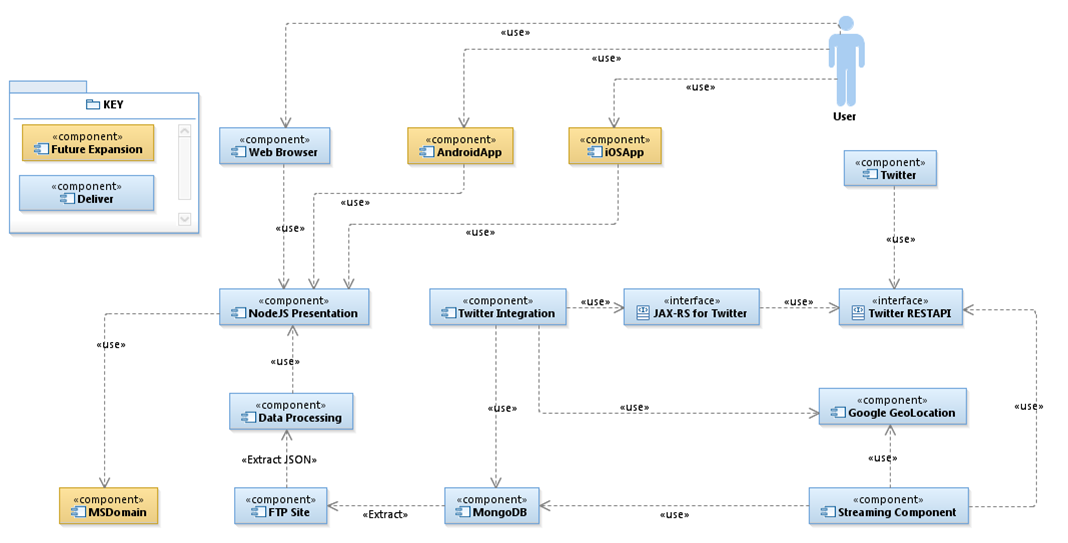
\includegraphics[width=1.0\linewidth]{HLD1}}
			\caption{High Level Component Model.}
			\label{fig:speciation}
		\end{figure}
	
	The table below provides a descriptive detail of all the key components that make-up the solution from data acquisition through to visualization.
	\begin{center}
		\begin{tabular}{ | l | p{12.7cm} |}
			\hline     	
			\textbf{Component} & \textbf{Key Function of Component} \\
			\hline
			Twitter & This component is the key provider of social media data for analysis and processing based on topics subscribed to. For this project, it was decided that topics subscribed to be centered around top political parties in the US and RSA elections.\\
			\hline
			TwitterRESTAPI & Twitter exposes a REST API for those interested in its publicly available data to integrate into their systems and acquire the data. Some limitations around how much data can be retrieved at any given time are imposed.\\
			\hline
			JAX-RS for Twitter & This solution, through this project shall deliver an interface based on JAVA API for XML Representational State service in order to integrate into Twitter for the acquisition of history data based on a date range.\\
			\hline
			Twitter Integration & This component is responsible for integrating into Twitter, orchestrating the validation and resolution of location information to Geographical Co-ordinates where location details are available as part of Twitter user preferences and persisting all the data on MongoDB.\\
			\hline
			Streaming Component & The standalone, windows based component shall also provide the same functionality as the Twitter Integration component; however, in this case, data being acquired shall be fresh data, streamed live as it happens.\\
			\hline
			MongoDB & This open source database was used for storing all the Big Data acquired from Twitter, both history data and online streaming data.\\
			\hline
			FTP Site & Periodically, a job shall be run to extract the data in the database and transfer it to the in JSON files for further processing on the Raspberry Pi cluster.\\
			\hline
			Data Processing & This component is dedicated to doing all the number crunching using Apache Spark while applying principles of MapReduce to ensure that all the Big Data is split and shared amongst all the Raspberry Pi cluster worker nodes.\\
			\hline
			Node.JS Presentation & This component shall read all the processed data and render it in a Web Browser in a manner that tries to communicate to the user the sentiments of potential voters for the upcoming 2016 elections in both the United States and South Africa.\\
			\hline
			Web Browser & The user interacts with the data using the Web Browser.\\
			\hline
			User & It is important to note that the user in this instance represent both the end-user who is interested in the elections analytics from Twit-Con-Pro and the admin-user who is responsible for the initial setting up of topics that are to be subscribed to.\\
			\hline
		\end{tabular}
	\end{center}
	
	\subsection{Operational Model: Infrastructure Design}
	
	As the title of the report suggests, this project is envisaged to leverage the use of low cost, commodity hardware in order to make a case for participating in Big Data projects without having to rely on big budgets and enterprise platforms.
	\\
	\\
	The below diagram depicts the production view of the end-to-end solution. In this diagram, it can be shown that the solution was running at completely separate geographical locations, even though at the heart of it (the number crunching and data analysis) all the nodes participating in the cluster were co-located at one geographical area.
	
		\begin{figure}[H] % Example image
		\center{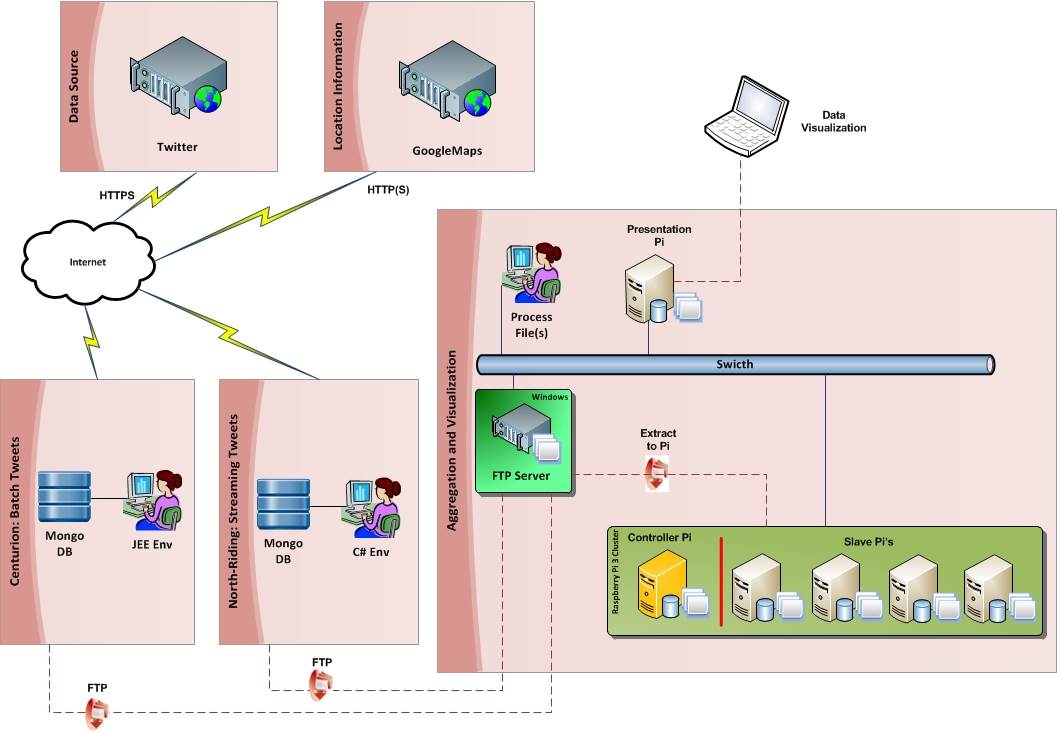
\includegraphics[width=1.15\linewidth]{OM1}}
			\caption{Operational Model: Phyical}
			\label{fig:speciation}
		\end{figure}
	
	The breakdown of the solution at an operational level was as follows for the production environment:
	
	\begin{itemize}
		\item \textbf{History\ Batch Data -} All batch data acquisitions from Twitter will be based in Centurion. Data acquired from Twitter shall be persisted in a MongoDB locally in that physical geographic are to avoid latency.
		\item \textbf{Streaming Data -} Streaming data shall be processed from the North-Riding location while data persistence is done locally to that site using MongoDB as well.
		\item \textbf{Aggregation and Visualization -} Most of the data "heavy-lifting" and number crunching shall happen using a cluster of Raspberry Pi's which are a very small pocket-sized "servers". The location information has been deliberately left out in this scenario because this part of the solution has been designed with high-mobility in mind.
	\end{itemize}
	
	%	CONCLUSION
	
	\section{Conclusion} % Major section
	
	All this hardware and software is available to anybody interested in Big Data processing.\\
	
	The hardware is cheap and the software is free.\
	
	The learning curve in the beginning can be quite steep but is ultimately very rewarding in terms of what can be achieved with so little financial investment.
	
	
	
	
	\newpage
	
	%----------------------------------------------------------------------------------------
	%	BIBLIOGRAPHY
	%----------------------------------------------------------------------------------------
	
	\begin{thebibliography}{99} % Bibliography - this is intentionally simple in this template
		
		\bibitem 1. S. Madam. From Databases to Big Data. IEEE Computer Society, 2012.
	
		%\newblock 
		
		\bibitem 2. V. Kumar, R. Yuvaraj, C. Anusha. Effective Distribution of Large Scale Datasets Clustering Based on MapReduce. 2016.

		
	\end{thebibliography}
	
	\section{Appendices}
	
	\subsection{Appendix A: Individual Time-Sheet}
		
	\subsection{Appendix B: Lifecycle Methodology}
	
	\subsubsection{Inception Phase}
	
	\subsubsection{Elaboration}
	
	\subsubsection{Construction}
	
	\subsubsection{Transition}
	
	\subsection{Appendix C: Non-Functional Requirements}
	
	\subsection{Appendix D: Solution Sequence Diagrams}
		
		\begin{figure}[H] % Example image
			\center{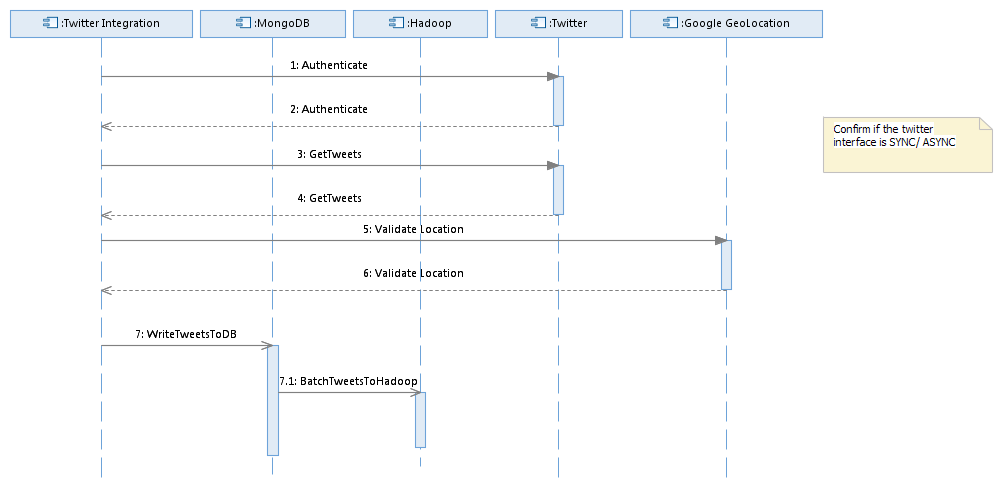
\includegraphics[width=1.15\linewidth]{SD_JEE}}
			\caption{Sequence Diagram: Data Integration - History}
			\label{fig:speciation}
		\end{figure}
		
	\subsection{Appendix E: List of Tools and Techniques}
	
	%----------------------------------------------------------------------------------------
	
\end{document}